% SPDX-License-Identifier: Apache-2.0
\documentclass[11pt,a4paper]{article}
\usepackage[T1]{fontenc}
\usepackage[utf8]{inputenc}
\usepackage{lmodern,microtype}
\usepackage[margin=26mm]{geometry}
\usepackage{amsmath,amssymb,mathtools}
\usepackage{graphicx,booktabs,tabularx,array}
\usepackage{xcolor,listings,enumitem,needspace}
\usepackage[numbers,sort&compress]{natbib}
\usepackage{hyperref}
\usepackage{bookmark}
\hypersetup{colorlinks=true,linkcolor=blue!45!black,citecolor=blue!45!black,
 urlcolor=blue!45!black,pdftitle={jacobsrays: ordered voxel intersections},
 pdfauthor={jacobsrays contributors}}
\definecolor{codebg}{RGB}{246,248,250}
\lstset{basicstyle=\ttfamily\small,backgroundcolor=\color{codebg},
 frame=single,rulecolor=\color{black!15},breaklines=true,
 columns=fullflexible,keepspaces=true,showstringspaces=false,
 aboveskip=10pt,belowskip=10pt,xleftmargin=5pt,xrightmargin=5pt,
 keywordstyle=\color{blue!55!black},commentstyle=\color{black!60}}
\setlength{\parskip}{4pt}
\setlength{\parindent}{0pt}
\widowpenalty=10000
\clubpenalty=10000
\setlength{\emergencystretch}{2em}
\renewcommand{\bibfont}{\small\raggedright}
\newcolumntype{Y}{>{\raggedright\arraybackslash}X}
\setlist{itemsep=2pt,topsep=4pt}
\newcommand{\dd}{\,\mathrm{d}}
\newcommand{\tr}{\operatorname{tr}}
\newcommand{\pack}{\operatorname{pack}}
\newcommand{\code}[1]{\texttt{\detokenize{#1}}}
\newcommand{\repo}[2]{\href{https://github.com/billlion/jacobsrays/blob/854c6aa60d64be38619be6d268ceb6b7b56da5f7/#1}{\code{#2}}}
\newcommand{\atomiclink}{\href{https://github.com/billlion/jacobsrays/pull/7}{PR~7}}
\title{\texttt{jacobsrays}: ordered voxel intersections\\for tensor tomography and transport}
\author{Project documentation --- user and methods guide}
\date{Draft, 28 October 2026}
\begin{document}
\maketitle
\begin{abstract}
Ray--voxel intersections provide a reusable geometric foundation for scalar
and tensor tomography and for transport equations along rays. This guide
describes a small C++11 implementation with Python and MATLAB interfaces,
including integration with the Core Imaging Library (CIL). It specifies the
coordinate and tensor conventions, explains how the same intersection
weights produce matched forward and adjoint operators, and shows why
ordered intervals are needed for non-commuting matrix transport. We document
the connection to David Szotten's earlier code, independent validation
against analytic calculations and ASTRA, and measured CPU performance,
including an optional OpenMP atomic adjoint and experimental cached
oneMKL products. Worked examples distinguish
discrete consistency from continuum accuracy. This is practical software
documentation, not a claim of a new ray-tracing algorithm or a general
solution to tensor or non-Abelian inverse problems.
\end{abstract}

\textbf{Repository:} \url{https://github.com/billlion/jacobsrays}.
The implementation is Apache-2.0 licensed. This draft describes main revision
\href{https://github.com/billlion/jacobsrays/commit/854c6aa60d64be38619be6d268ceb6b7b56da5f7}{\code{854c6aa}}
(package version 0.1.0), including the optional atomic adjoint merged in
\atomiclink. The atomic-adjoint measurements were made on revision
\href{https://github.com/billlion/jacobsrays/commit/f6464f3cb3565c8a2f0021138e96efcd0e7958c0}{\code{f6464f3}} before that merge.
Section~\ref{sec:csf3-mkl} adds later CSF3 measurements of a benchmark-only
oneMKL adapter; their raw records and provenance limitations are documented
in \path{benchmarks/csf3/README.md}.

\subsection*{Reading this guide}
For a first calculation, read the coordinate contract in
Section~\ref{sec:geometry} and the examples in Section~\ref{sec:examples}.
The Python listings are complete executable files; the MATLAB and CIL
sections point to full examples in the repository.

For a new tensor or transport model, start with the operator conventions
in Section~\ref{sec:tensors}. In particular, tensor packing, transverse
trace and multiplication order are part of the numerical model.

For assessing results or choosing an implementation strategy, consult the
validation evidence in Section~\ref{sec:validation} and the measured time
and memory tradeoffs in Section~\ref{sec:speed}. The limitations accompany
each experiment so that reproducible consistency checks are not mistaken
for reconstruction accuracy claims.

Appendix~\ref{app:exact} starts a verification study with a precise
specification and written exact-arithmetic correctness proof of the
traversal. It introduces the proof terminology and a worked example;
it is not yet a machine-checked or floating-point verification.

\clearpage
\begingroup
\small
\tableofcontents
\endgroup
\clearpage

\section{Why a small ray--voxel library?}
Many imaging models share a geometric question: which cells of a Cartesian
grid does a straight ray cross, and for how long does it remain in each?
For a piecewise-constant scalar field, these lengths are the coefficients
of a discrete X-ray transform. For a tensor field, the same coefficients
can be combined with contractions or projections depending on the ray
direction. For a transport equation, the entry and exit points define
successive integration intervals. Keeping the geometry separate makes it
possible to change the measurement model without rewriting traversal.

This separation is useful in experimental tensor imaging: one may need a
new tensor contraction, a polarisation readout, an unusual set of rays, or
the derivative of a nonlinear forward model. A compact, inspectable CPU
kernel also provides a reference against which more specialised
implementations can be checked. It does not replace a complete imaging
toolbox, detector model or reconstruction method.

The main supported uses are the scalar X-ray transform, the longitudinal
ray transform (LRT) of symmetric tensors, and the full transverse ray
transform (TRT) of symmetric rank-two tensors. The truncated transverse ray
transform (TTRT), used in linearised photoelastic tomography, can be built
from the same geometry and transverse projection. The distinction between
full and truncated data matters: the latter removes the transverse trace.
Section~\ref{sec:tensors} gives the precise conventions and implementation
status. ORT is a proposed further application; this draft does not assign
it a definition or claim an implementation. A public specification and
validation example are needed before adding it to the API.

Non-Abelian ray transforms require additional information that scalar
matrix storage need not preserve: \emph{travel order}. Rotations or other
matrix propagators generally do not commute, so changing the order of
encountered voxels changes the result. Polarimetric neutron imaging is a
concrete application~\cite{desai2020,sales2018}. The package returns ordered
intervals directly rather than requiring users to infer order from a sparse
matrix.

\subsection{Relation to ASTRA, TIGRE and CIL}
ASTRA~\cite{astra2016} and TIGRE~\cite{tigre2016} provide mature tomography
infrastructure and GPU projectors. They are natural choices for many large
scalar imaging problems. \code{jacobsrays} currently supplies a CPU kernel,
explicit segment geometry, and a small set of scalar and tensor operators.
Its useful distinguishing feature here is access to ordered cell intervals
and a common traversal for custom forward models.

Comparisons must specify a projector, not just a toolbox name. ASTRA's 2D
CPU \code{line} projector uses intersection lengths; its \code{linear}
projector uses a Joseph-type interpolation model~\cite{astraprojectors}.
TIGRE also exposes different forward and backward models. For example, the
documented CIL TIGRE adapter distinguishes Siddon and interpolated forward
projection, and describes its matched adjoint weights as approximately
matching the interpolated method~\cite{ciltigre}. This does not establish
an exact transpose for every possible pairing. Independent numerical
checks should follow the chosen configuration.

CIL~\cite{cil2021} provides optimisation algorithms and data containers
into which a new operator can be inserted. Our adapter therefore implements
CIL's operator interface directly, without requiring ASTRA or TIGRE as a
backend. No comparative GPU speed result is claimed in this guide.

\section{History and provenance}
\label{sec:history}
The underlying traversal belongs to the Siddon/Jacobs family.
Siddon~\cite{siddon1985} describes the grid through its planes rather than
testing every voxel separately. Jacobs et al.~\cite{jacobs1998} describe
an efficient calculation of the radiological path. The present implementation
merges the ordered sequences of plane crossings; it does not claim a new
geometric algorithm.

David Szotten developed a MATLAB-wrapped implementation at Manchester;
the source preserved in \code{LRTinMatlab} carries 2005--2008 attribution.
His thesis concerns limited-data X-ray and polarised-light tomography,
including the TTRT~\cite{szotten2011}. The university catalogue records the
award on 3 December 2010, while the later papers cite the thesis as 2011;
the bibliography follows those citations and records this distinction.

The historical connection is documented in several public sources:
\begin{itemize}
\item The 2006 MIMS preprint by Szotten, Lionheart and Tomlinson describes
using Jacobs intersection lengths to construct scalar, transverse and
truncated transverse matrices. It also describes accumulating the transpose
ray by ray when storing the full matrix is impractical~\cite{szotten2006}.
It is cited here as a preprint, not as a subsequently published journal
article.
\item Desai and Lionheart's three-axis TRT reconstruction paper provides
the published tensor phantom used in our slice example. Its numerical
method section explicitly follows the ray integration procedure in
Section 5.1.4 of Szotten's thesis~\cite{desai2016}. The MATLAB research-code repository
preserves the older ray implementation~\cite{lrtmatlab}.
\item Section 7 of Desai et al.'s polarimetric-neutron paper explicitly
states that its forward solver used the Jacobs method as implemented in
Szotten's thesis, modified to return voxel encounter order. Voxelwise
constant magnetic fields then give successive rotation matrices along
the ray~\cite{desai2020}. The experimental context is described by
Sales et al.~\cite{sales2018}.
\end{itemize}

This history explains the present emphasis on both lengths and ordering.
The new C++ implementation was written afresh after an audit of the older
interface and behaviour. The inspected legacy tree did not contain a
licence granting redistribution of its code; no legacy source is bundled
or relicensed. The repository's \code{NOTICE} records the intellectual
provenance and development assistance.

The audit found practical reasons to make the conventions explicit. In the
old implementation, non-square grids could receive an incorrect linear
index, the final partial segment could be mishandled, and some reported
weights were parameter intervals rather than physical lengths. A MATLAB
sparse-sizing idiom could overwrite a genuine final coefficient. The
legacy help text also disagreed with the implementation about the grid
offset. These are recorded with small examples in
\repo{docs/legacy-audit.md}{docs/legacy-audit.md}; they are not reasons to
treat all historical numerical results as invalid. The compatibility
wrapper preserves the old calling convention while using the corrected,
documented geometry.

\section{Geometry, storage and the traversal kernel}
\label{sec:geometry}
\subsection{Coordinate contract}
Let the grid have shape $(n_x,n_y,n_z)$, positive spacing
$h=(h_x,h_y,h_z)$ and lower corner $o$. Voxel $(i,j,k)$ is
\[
 [o_x+ih_x,o_x+(i+1)h_x)\times
 [o_y+jh_y,o_y+(j+1)h_y)\times
 [o_z+kh_z,o_z+(k+1)h_z).
\]
The zero-based linear index is $i+n_x(j+n_y k)$. Thus $x$ is the fastest
varying coordinate. Two-dimensional grids use the same rules with the
$z$ coordinate omitted at the public interface.

Inputs are finite segments
\begin{equation}
 x_r(t)=a_r+t(b_r-a_r),\qquad 0\leq t\leq1.
 \label{eq:segment}
\end{equation}
Endpoints need not lie outside the grid. To approximate an infinite line
through the object, choose endpoints enclosing its entire intersection
with the grid. If an emitted interval is $[t_0,t_1]$, its physical length is
\begin{equation}
 \ell=(t_1-t_0)\lVert b_r-a_r\rVert_2.
 \label{eq:length}
\end{equation}
The parameters themselves are dimensionless, not arclengths.

\begin{table}[htbp]
\centering\small
\begin{tabularx}{\linewidth}{@{}lYY@{}}
\toprule
Convention & Python & MATLAB \\
\midrule
Geometry arguments & $(n_x,n_y[,n_z])$, xyz endpoints & Same \\
Image array shape & $(n_z,n_y,n_x)$ or $(n_y,n_x)$ & $[n_x,n_y,n_z]$ or $[n_x,n_y]$ \\
Linear storage & C order; x fastest & Column major; x fastest \\
Indices and offsets & Zero based & One based \\
Scalar range & One number per input ray & One number per input ray \\
Empty/missing rays & Repeated offsets; zero matrix rows & Same meaning \\
\bottomrule
\end{tabularx}
\caption{Coordinate and storage conventions. Array shape reversal is deliberate;
it does not reverse the physical coordinate axes.}
\end{table}

A parallel ray on an internal cell plane belongs to the higher-index cell.
The lower exterior face is included and the upper exterior face excluded.
Point tangencies, misses and zero-length segments emit no positive-length
intervals. These boundary choices have measure zero in continuum theory
but are essential for reproducible discrete tests.

\subsection{Streaming the intersections}
The computational core is
\repo{include/jacobsrays/traverse.hpp}{include/jacobsrays/traverse.hpp}.
It is a header because the central \code{walk<Emit>} routine is templated
on its output action. Keeping its definition visible lets the compiler
specialise and inline different actions without a virtual call at every
intersection. Header implementation is a C++ design choice, not an
assumption that headers execute faster.

Conceptually the traversal performs the following operations:
\begin{enumerate}
\item Clip the segment to the grid box by intersecting its parameter interval
with the coordinate slabs. Return if there is no positive-length overlap.
\item Find the cell at entry and the next grid-plane crossing for each axis.
An axis parallel to the ray contributes no finite next crossing.
\item Take the earliest next crossing, or the clipped segment exit if sooner.
Emit the current cell index, physical length, and entry/exit parameters.
\item Advance every axis tied at that crossing, update its next plane, and
continue until exit.
\end{enumerate}
This merges two or three monotone crossing sequences without sorting a
list of all crossings. Work is $O(K_r)$ for $K_r$ crossed cells, with
$O(1)$ traversal workspace per ray. Next crossing parameters are recomputed
from integer plane positions to limit cumulative drift. Exact ties advance
all tied axes. Numerically near-tied crossings can produce very short
positive intervals; the code does not silently merge them using an
arbitrary absolute tolerance. Reversal is consequently checked numerically,
not promised to be bitwise identical.

Finite inputs, representable grid extents and integer index ranges are
checked. There is no absolute small-direction cutoff such as $10^{-8}$;
such a cutoff would depend on the user's physical units. Standard compiler
optimisation is appropriate. Unrestricted fast-math transformations are
not assumed because the algorithm uses finite-value and infinity semantics.

\begin{figure}[htbp]
\centering
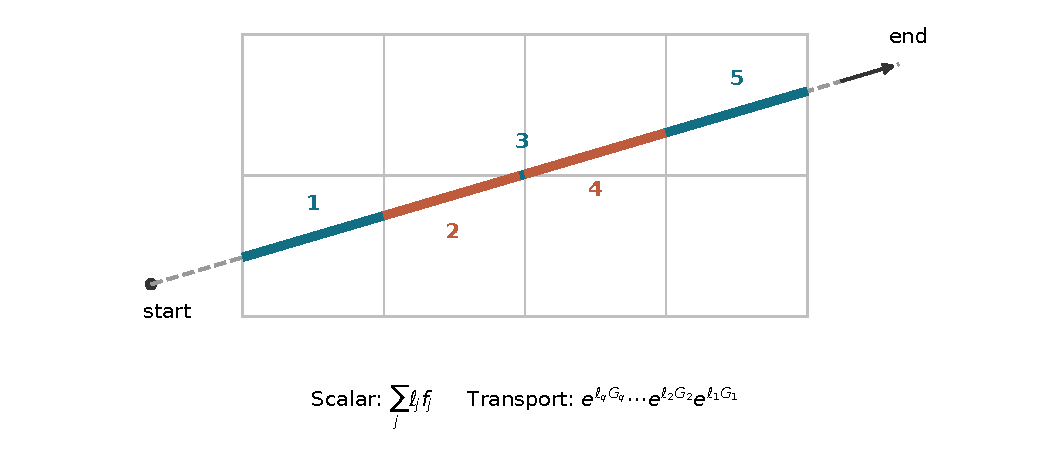
\includegraphics[width=.88\linewidth]{figures/ordered-ray.pdf}
\caption{A finite segment clipped to a grid, with intervals numbered in travel
order. Scalar projection sums length-weighted values. Matrix transport
applies the first propagator first, placing later factors to its left for
the convention $U'=GU$. Cell numbers in the sketch are encounter labels,
not linear storage indices.}
\end{figure}

\subsection{Retain paths or recompute them?}
\code{trace} returns ragged ordered arrays: \code{offsets}, \code{indices},
\code{lengths}, \code{t_enter} and \code{t_exit}. Entries for ray $r$ are
selected by successive offsets, in start-to-end order. Native batch tracing
counts intersections and then fills exactly sized arrays in a second pass.
The Python wrapper releases the GIL during native computation.

For $K$ total intersections and $R$ rays, the returned arrays occupy
$32K+8(R+1)$ bytes with 64-bit indices and double precision lengths and
parameters. This excludes object headers and input geometry. Batching rays
limits this storage. Conversion to a scalar sparse matrix discards the
entry/exit parameters, and subsequent sparse operations may reorder
columns. Use the original paths for transport ODEs.

The scalar \code{RayTransform} instead retraces rays on each application,
avoiding persistent intersection storage. Python tensor operators cache
one scalar CSR matrix, and combine it with small direction-dependent
operations. MATLAB exposes sparse matrices. These choices trade setup
cost and memory against repeated-iteration speed; no single choice wins
for every acquisition.

\section{Operators, adjoints and tensor conventions}
\label{sec:tensors}
\subsection{Scalar projection and a matched backprojector}
For piecewise-constant voxel values $x_i$, define
\begin{equation}
 A_{ri}=\operatorname{length}(\text{segment }r\cap\text{voxel }i),
 \qquad (Ax)_r=\sum_i A_{ri}x_i,
 \qquad (A^\mathsf{T}y)_i=\sum_r A_{ri}y_r.
 \label{eq:transpose}
\end{equation}
The native forward callback adds $\ell x_i$ to one ray output; the
backprojection callback adds $\ell y_r$ to one voxel output. Both call the
same traversal with the same endpoints. Backprojection does not reverse
the ray and does not substitute another interpolation or quadrature rule.

CIL's \code{JacobProjector.adjoint} method is defined in
\path{python/jacobsrays/cil.py}. It calls the main Python module's
\code{RayTransform.adjoint} method, defined in
\path{python/jacobsrays/__init__.py}. The native backprojector in
\code{src/python.cpp} then invokes \code{walk} in \code{traverse.hpp}.
Tensor adjoints follow their
cached scalar matrix transpose instead of this matrix-free native path.

This is a \emph{matched discrete transpose}, up to floating-point arithmetic.
It is the adjoint for ordinary Euclidean array dot products. For weighted
inner products with positive definite matrices $W_X$ and $W_Y$, the
corresponding adjoint is $W_X^{-1}A^\mathsf{T}W_Y$. Voxel volumes, detector
areas and angular quadrature weights are not inserted automatically.

An unmatched pair uses a backward operator $B\ne A^\mathsf{T}$. Such pairs
can be useful computationally, but replacing $A^\mathsf{T}$ by $B$ changes
the algebra of an iterative method: $BA$ need not be symmetric positive
semidefinite and $B(Ax-y)$ need not be the least-squares gradient. The usual
CGLS reasoning therefore no longer applies. Perturbation and convergence
analysis, and methods designed for unmatched pairs, are discussed in
\citet{elfving2018,hansen2022}. Neither hardware texture interpolation nor
GPU execution alone establishes that a particular pair is unmatched;
the actual weights and their transpose must be examined.

A matched pair still does not guarantee an accurate or unique reconstruction.
Nullspaces, acquisition coverage, noise, discretisation and regularisation
remain properties of the inverse problem.

\subsection{LRT and orthonormal packing}
For a symmetric rank-$m$ tensor field $f$ and an oriented unit ray direction
$u$, the LRT is
\begin{equation}
 (I_m f)(r)=\int_r f(x)[u,\ldots,u]\dd s.
\end{equation}
Let $\alpha=(\alpha_1,\ldots,\alpha_d)$ with $|\alpha|=m$, and
$c_\alpha=m!/\alpha!$. Store the tensor component as
$x_\alpha=\sqrt{c_\alpha}f_\alpha$, and define
$w_{r\alpha}=\sqrt{c_\alpha}u_r^\alpha$. Then
\begin{equation}
 (Lx)_r=\sum_\alpha w_{r\alpha}(Ax_\alpha)_r,
 \qquad
 (L^\mathsf{T}y)_\alpha=A^\mathsf{T}(w_{\cdot\alpha}\odot y).
\end{equation}
This orthonormal packing makes an ordinary component dot product equal to
the tensor Frobenius product, including the multiplicities of off-diagonal
components. In 3D at rank two it is
\begin{equation}
 \pack(F)=(F_{11},\sqrt2F_{12},\sqrt2F_{13},
                   F_{22},\sqrt2F_{23},F_{33}).
 \label{eq:pack}
\end{equation}
In 2D it is $(F_{11},\sqrt2F_{12},F_{22})$.
\code{TensorRayTransform} implements these formulas in 2D and 3D for
nonnegative integer rank; its \code{exponents} attribute records the
component order. Reversing the endpoints changes the LRT by $(-1)^m$.
The familiar potential-field nullspace of the continuum LRT is not removed
by this discretisation~\cite{sharafutdinov1994}.

\subsection{Full rank-two TRT, trace tests and TTRT}
Let $P_u=I-uu^\mathsf{T}$. The implemented full TRT is
\begin{equation}
 (Jf)(r)=\int_r P_{u_r}f(x)P_{u_r}\dd s.
 \label{eq:trt}
\end{equation}
\code{TransverseRayTransform} uses the packing in~\eqref{eq:pack} in both
domain and range. Its 3D input has shape $(6,n_z,n_y,n_x)$ and output has
shape $(R,6)$. The six output entries encode only three independent
transverse components; retaining a Cartesian representation avoids an
arbitrary detector-frame choice. If $E$ contains two orthonormal transverse
detector axes, the detector matrix is $E^\mathsf{T}(Jf)E$.

For each ray the map $F\mapsto P_uFP_u$ is self-adjoint in the Frobenius
product. Thus the discrete adjoint applies this map to the input tensor
data and backprojects each resulting component with $A^\mathsf{T}$.
It is defined even for data that are not already transverse. Small
per-ray projectors and one scalar CSR matrix are retained; a dense block
tensor matrix is not assembled in Python.

Two useful identities follow directly:
\begin{equation}
 \tr(Jf)=X(\tr f)-I_2f,
 \qquad
 J(\phi I)=(X\phi)P_u.
 \label{eq:trace}
\end{equation}
Here $X$ denotes the scalar line integral along the same ray. Consequently
$\tr J(\phi I)=(d-1)X\phi$. These test the retained transverse trace as well
as the component packing. The full TRT is relevant to published tensor
imaging models including diffraction tomography of strain~\cite{lionheart2015}
and the reconstruction analysis of \citet{desai2016}.

For rank two in 3D, define the transverse trace-free map
\begin{equation}
 Q_u(F)=P_uFP_u-\frac{\tr(P_uFP_u)}{2}P_u.
 \label{eq:ttrt}
\end{equation}
The TTRT integrates this quantity~\cite{szotten2006,lionheart2009}.
The divisor is the transverse dimension, two, not the ambient dimension
three. Isotropic fields are invisible: $Q_u(\phi I)=0$.
``Truncated'' in this usage concerns the transverse trace; it does not
mean a spatially truncated field of view. The current API implements the
full TRT, not a separate TTRT class. A future adapter can apply $Q_u$ to
the full TRT output and use the same self-adjoint projection in its
backward map. This guide does not introduce unpublished Fourier inversion
formulas or equate three-axis data with complete directional data.

\subsection{Ordered transport and non-Abelian models}
\label{sec:transport}
Suppose a matrix propagator satisfies
\begin{equation}
 \frac{\dd U}{\dd s}=G(x(s),u)U(s),\qquad U(s_{\mathrm{entry}})=I,
\end{equation}
where $s$ is physical arclength. With constant generator $G_j$ in the
$j$th encountered voxel and interval length $\ell_j$,
\begin{equation}
 U_{\mathrm{exit}}=
 e^{\ell_q G_q}\cdots e^{\ell_2 G_2}e^{\ell_1 G_1}.
 \label{eq:product}
\end{equation}
The latest factor is leftmost for this ODE convention. In general this is
not $\exp(\sum_j\ell_jG_j)$. The geometric traversal is exact for the
specified cells; matrix-exponential evaluation has numerical error, and
approximating a smooth field by voxel constants has model error.

The example \code{examples/nonabelian_transport.py} implements this product
with SciPy matrix exponentials. It is a generic forward-model building
block, not a complete neutron or optical instrument model. For variable
within-voxel coefficients, recover the physical entry/exit points from
\eqref{eq:segment} and use an ODE solver on each interval. A connection
uses a direction-dependent generator: reversal changes both traversal
order and the contracted generator sign. Reversing endpoints alone for an
orientation-independent $G(x)$ does not generally produce inverse transport.

The forward map in~\eqref{eq:product} is nonlinear in the generators. Its
linearisation contains products before and after each perturbation; the
scalar backprojector is not automatically its Jacobian adjoint. That
derivative and its tests belong in any future nonlinear reconstruction
implementation. This separation follows the physical motivation of the
polarimetric-neutron work without claiming to reproduce its full inversion.

\section{Interfaces and worked use}
\label{sec:examples}
\subsection{Python: paths, sparse matrices and matrix-free projection}
From a checkout with a C++ compiler and Python 3.10 or newer:
\par\noindent\begin{minipage}{\linewidth}
\begin{lstlisting}[language=bash]
python -m pip install '.[scipy]'
\end{lstlisting}
\end{minipage}\par
NumPy is the mandatory runtime dependency. SciPy is needed for sparse
matrices, tensor operators, iterative solves and the matrix-exponential
example. The following is a complete small scalar example:
\par\noindent\begin{minipage}{\linewidth}
\lstinputlisting[language=Python]{snippets/scalar.py}
\end{minipage}\par
It prints indices $0,1,2$, three unit lengths, and the scalar projection
$3$. The scalar API uses real double-precision arrays. Complex generators
can be used in the Python transport example, but the scalar and tensor
projector APIs do not currently accept complex image data.

\Needspace{22\baselineskip}
\subsection{Python: a tensor with a known transverse trace}
The following uses $f=\phi I$ on a small 3D grid. It checks the trace
identity without constructing a full tensor system matrix:
\par\noindent\begin{minipage}{\linewidth}
\lstinputlisting[language=Python]{snippets/trt_trace.py}
\end{minipage}\par
For more varied fields, \code{examples/tensor_trt.py} uses a spatial mask
and an anisotropic tensor, checks transversality and the adjoint identity,
and can reconstruct with CIL. \code{examples/tensor_lrt.py} demonstrates
the longitudinal operator and its rank-dependent packing.

\subsection{MATLAB and compatibility with older scripts}
\par\noindent\begin{minipage}{\linewidth}
\begin{lstlisting}[language=Matlab]
addpath('matlab');
build_jacobsrays;
test_jacobsrays;
test_trt;
p = jacobsrays([3 2], [-1 .5], [4 .5]);
A = jacobsrays_matrix(p);
x = ones(3,2);
y = A*x(:);
xadj = reshape(A'*y, [3 2]);
k = p.offsets(1):p.offsets(2)-1;
disp([p.indices(k), p.lengths(k)]);
\end{lstlisting}
\end{minipage}\par
The MEX layer uses the same C++ header. Inputs are full real double arrays;
the path indices and offsets returned to MATLAB are one based.
\code{jacobsrays_matrix} preserves empty rows and the requested full shape,
including a zero-ray matrix. MATLAB's sparse transpose supplies the matched
scalar adjoint.

For rank-two TRT, \code{jacobsrays_trt_matrix} explicitly builds the block
sparse matrix $T$. With voxel components stored as an $N\times c$ matrix
$F$, and ray components as an $R\times c$ matrix $Y$, use
\par\noindent\begin{minipage}{\linewidth}
\begin{lstlisting}[language=Matlab]
[T, paths] = jacobsrays_trt_matrix(shape, starts, ends, spacing, origin);
Y = reshape(T*F(:), size(starts,1), size(F,2));
Fadj = reshape(T'*Y(:), prod(shape), size(F,2));
\end{lstlisting}
\end{minipage}\par
Here $c=6$ in 3D and $c=3$ in 2D, with the orthonormal components already
packed. MATLAB vectorisation is component-major in both spaces; Python's
TRT output is an $R\times c$ C-order array. Do not transfer flattened
tensor arrays between languages without respecting this distinction.
The explicit 3D tensor matrix can have up to 36 entries per scalar
intersection, so it is intended for modest problems. A complete runnable
MATLAB example is \code{matlab/example_trt.m}.

The compatibility function \code{mod_jacobs_ray3d_multiple} preserves the
old signature, including ordered \code{'internal'} triples. Its offset
means the lower grid corner, matching the legacy implementation rather
than the contradictory old help text. Put the new MATLAB directory first
on the search path and check geometry conventions when porting scripts.

\subsection{CIL solvers}
CIL is installed separately using its own instructions~\cite{cildocs}.
The adapter provides \code{direct}, \code{adjoint} and optional \code{out}
arguments. Scalar \code{JacobProjector} maps a single-channel
\code{ImageGeometry} to a \code{VectorGeometry} with one entry per supplied
ray. It currently requires the default spatial dimension labels and no
singleton spatial dimensions. It does not infer rays from a CIL
\code{AcquisitionGeometry}.

With an image geometry \code{ig}, explicit endpoints and compatible data,
the central CGLS calls are:
\par\noindent\begin{minipage}{\linewidth}
\begin{lstlisting}[language=Python]
from cil.optimisation.algorithms import CGLS
from jacobsrays.cil import JacobProjector
operator = JacobProjector(ig, starts, ends)
solver = CGLS(initial=ig.allocate(0, dtype=np.float64),
              operator=operator, data=data)
solver.run(30, verbose=0)
image = solver.solution
\end{lstlisting}
\end{minipage}\par
\code{examples/cil_cgls.py} supplies the complete geometry and data setup.
Its recorded noiseless demonstration reached a relative data residual of
about $1.68\times10^{-4}$ after 30 iterations. This is an example outcome,
not a general convergence guarantee or a recommended stopping rule for
noisy measurements.

\code{TensorJacobProjector} has a block-image domain and a scalar-vector
range. The TRT adapter, \code{TransverseJacobProjector}, uses component
blocks in both domain and range. Run
\par\noindent\begin{minipage}{\linewidth}
\begin{lstlisting}[language=bash]
python examples/cil_cgls.py
python examples/tensor_lrt.py
python examples/tensor_trt.py --cil
python examples/nonabelian_transport.py
\end{lstlisting}
\end{minipage}\par
The CIL adapter is imported only when requested. Tensor operators use
cached scalar matrices; they do not route their adjoints through the
native atomic scalar implementation.

\section{Validation: what has been checked?}
\label{sec:validation}
Validation is layered because a dot-product test alone can pass for a
consistently wrong forward model. Conversely, comparing two legitimate
but different discretisations need not give roundoff-level agreement.
\begin{table}[htbp]
\centering\small
\begin{tabularx}{\linewidth}{@{}p{.22\linewidth}YY@{}}
\toprule
Layer & Evidence & Main limitation \\
\midrule
Traversal & 4,000 random 2D/3D segments against an independent plane-enumeration
oracle; hand cases and edge cases & Finite sampling of floating-point inputs \\
Operator algebra & Sparse versus matrix-free results; transpose dot products;
LRT ranks 0--3 and TRT component checks & Shared geometry can hide common errors \\
Tensor physics & Independent per-voxel clipping and tensor formula;
transversality, isotropic and trace identities & Tests the stated model, not every instrument \\
External scalar code & ASTRA CPU line matrices, projections and adjoints;
CIL/ASTRA geometry integration & 2D, square pixels, single precision reference \\
Continuum example & Analytic Gaussian line integrals and separate numerical
quadrature; slice reconstruction & Specific phantom and fixed acquisition \\
Language bindings & C++ tests, Python tests, MATLAB MEX tests in CI & No claim of all compilers/platforms \\
\bottomrule
\end{tabularx}
\caption{Different checks answer different questions. Exact geometry,
adjointness, physical modelling and inverse-problem accuracy are distinct.}
\end{table}

\subsection{Geometry and adjoint tests}
The Python reference oracle enumerates plane intersections and sorts them;
it does not reuse the streaming walk. Cases include anisotropic spacing,
offset origins, non-cubic grids, reversed and partial rays, simultaneous
crossings, parallel rays on boundaries, misses, tangencies, empty batches,
zero-length segments and invalid inputs. C++ tests exercise the standalone
header. Address and undefined-behaviour sanitizer checks have also been
used during development; this is not a claim of exhaustive verification.

For real arrays the adjoint identity is
$\langle Ax,y\rangle=\langle x,A^\mathsf{T}y\rangle$. A useful diagnostic is
\begin{equation}
 \varepsilon_{\rm adj}=
 \frac{|\langle Ax,y\rangle-\langle x,A^\mathsf{T}y\rangle|}
 {\lVert Ax\rVert\lVert y\rVert+\lVert x\rVert\lVert A^\mathsf{T}y\rVert},
 \label{eq:adjtest}
\end{equation}
with zero treated separately when the denominator vanishes. This avoids
dividing only by a dot product that may nearly cancel. Tests also compare
against explicit sparse products. TRT tests use arbitrary tensor data in
the adjoint, so an incorrect assumption that all input data are already
transverse is detectable.

The atomic extension adds high-contention tests: 16,384 identical rays
accumulate into the same four voxels using exactly representable unit
lengths and small integer data. Random anisotropic 2D/3D cases compare
serial, atomic and sparse results; CIL tests exercise \code{out} and CGLS.
At the tested PR revision the OpenMP suite had 29 passing tests; the serial
build had 25 passes and four OpenMP-only skips. Counts are a dated snapshot,
not a coverage metric. MATLAB tests run separately on GitHub Actions; no
local MATLAB installation was used to build this document.

\subsection{Independent comparison with ASTRA}
\label{sec:astra}
The external tests use ASTRA 2.5.0 CPU \code{line} and \code{line_fanflat}
projectors. The direct comparison includes six geometries, each with 29
angles and 41 detector samples, for 7,134 rays in total. Images have
$11\times8$ pixels, with square-pixel widths 1, 0.375 and 2.5 and shifted
windows. Full system matrices are compared before forward and transpose
products. ASTRA's row ordering and this package's physical $y$ convention
are reconciled explicitly; an asymmetric image helps expose accidental
flips. Separate CIL/ASTRA tests cover parallel and fan geometries,
detector orientation and angular offsets.

ASTRA's reference values are single precision; our traversal uses doubles.
The coefficient tolerance is $3\times10^{-4}$ times pixel width, with
relative $L^2$ tolerance $2\times10^{-5}$ for the corresponding projection
checks. The recorded worst coefficient discrepancy was approximately
$1.79\times10^{-4}$ pixel widths; forward and adjoint discrepancies were
of order $10^{-6}$ to $10^{-5}$. These tolerances apply to these tests,
not a bound for all geometries.

This comparison does not validate 3D external projectors, tensor
contractions, travel order, or GPU interpolation kernels. Non-square
pixels are excluded from the ASTRA CPU line reference comparison;
anisotropic geometry is instead checked by the independent internal oracle.
TIGRE is discussed as a relevant toolbox but has not yet been used as a
validation or timing reference in this repository.

\subsection{Slice-by-slice TRT: discrete consistency and continuum error}
\label{sec:slices}
If a ray lies in an $x_3$-constant plane, then $u_3=0$ and $P_ue_3=e_3$.
It follows for any symmetric field that
\begin{equation}
 (Jf)_{33}(r)=\int_r f_{33}(x)\dd s.
\end{equation}
Thus a scalar 2D reconstruction can recover this component on the plane
from these TRT data, subject to the usual sampling and inversion issues.
Choosing voxel-centre planes avoids inter-slice interpolation.

\code{examples/trt_slices.py} uses only the published $f_{33}$ component
from Table 1 of \citet{desai2016}. On $[-1,1)^3$ it is
\begin{align}
 f_{33}(x)={}&e^{-50\lVert x-(.5,-.5,-.5)\rVert^2}
              -e^{-50\lVert x-(.5,-.5,.5)\rVert^2}\nonumber\\
            &+e^{-50\lVert x-(.5,.5,.5)\rVert^2},
\end{align}
and is zero outside; the other tensor components are set to zero here.
This example does not reproduce the paper's full tensor phantom or
three-axis inversion algorithm.

Two layers centred at $x_3=\pm0.5$ contain $n\times n$ centre samples.
The default acquisition uses 90 angles over a half-turn with angular
offset 0.013 radians, and 129 detector offsets from $-1.45$ to $1.45$.
Three data sets are compared: the $33$ output of the voxel TRT, a separate
2D scalar projection of the samples, and analytic integrals of the
continuous Gaussian sum clipped to the cube and finite segments. The last
use error functions and are independently checked against adaptive
quadrature.

Each data set is inverted with the same scalar matrix and unregularised
LSMR, tolerances \code{atol=btol=1e-10} and at most 300 iterations. The
reference is the sampled continuous field, not voxel averages.
\begin{table}[htbp]
\centering\small
\begin{tabular}{@{}rccc@{}}
\toprule
Slice grid & Voxel/analytic data error & \multicolumn{2}{c}{Image error from analytic data}\\
 & relative $L^2$ & $x_3=-0.5$ & $x_3=+0.5$ \\
\midrule
$32\times32$ & 4.13\% & 2.79\% & 2.77\% \\
$64\times64$ & 1.48\% & 4.62\% & 5.32\% \\
\bottomrule
\end{tabular}
\caption{Recorded slice example (NumPy 2.3.5, SciPy 1.17.0).
Smaller forward modelling error does not imply a smaller unregularised
reconstruction error when acquisition sampling is held fixed.}
\end{table}

TRT and scalar voxel data agreed exactly in that run, as did their
reconstructions. Matched voxel-data image errors were approximately
$2\times10^{-9}$ and $2\times10^{-8}$ at the two resolutions. This is a
discrete consistency check, often called an inverse crime, rather than
independent evidence of continuum reconstruction accuracy. All default
solves stopped on tolerance before the iteration limit.

The analytic-data image errors increase under this refinement even though
the data discrepancy decreases. Fixed acquisition sampling, conditioning
and model mismatch can all affect the inverse result; this experiment does
not isolate them. Regularisation and controlled refinement of both image
and acquisition are needed for a convergence study. The small CI regression
therefore tests identities and solver consistency rather than imposing a
false monotonic error requirement.

\section{Speed, memory and parallel accumulation}
\label{sec:speed}
\subsection{Recorded scalar benchmark}
The recorded 26 October 2026 benchmark used Linux, an AMD EPYC 9V74 CPU,
GCC 13.3.0, Python 3.12.14 and NumPy 2.3.5. There were 20,000 segments on a
$64^3$ grid and 2,107,166 intersections. Times below are the best of five
warm repetitions and include per-call validation and output allocation.
CSR timings exclude construction of the matrix.
\begin{table}[htbp]
\centering\small
\begin{tabular}{@{}lrr@{}}
\toprule
Operation & Serial build (ms) & OpenMP, 4 threads (ms) \\
\midrule
Ordered paths, two passes & 46.42 & 9.90 \\
Matrix-free forward & 23.33 & 5.48 \\
Matrix-free adjoint, serial accumulation & 24.45 & 24.48 \\
Cached CSR forward & 1.63 & 1.62 \\
Cached CSR transpose & 1.94 & 2.08 \\
\bottomrule
\end{tabular}
\caption{Scalar benchmark before the atomic extension. The CSR operations
use SciPy and do not acquire a four-thread traversal merely because the
native extension was built with OpenMP.}
\end{table}
The ordered arrays occupied 67,589,320 bytes; the SciPy CSR matrix occupied
25,365,996 bytes in that run, including its 32-bit index arrays. CSR is
smaller because it omits the interval endpoints and uses narrower indices
for this problem. It also amortises geometry over repeated iterations.
The matrix-free method is useful when storage or changing ray geometry
makes caching undesirable.

A separate one-pass native comparison used 200,000 rays with
21,068,823 intersections. The legacy C traversal took 137.70 ms and the new
C++ traversal 164.20 ms, approximately 19\% longer. Intersection counts
and the recorded length checksum agreed for that geometry. This test
excludes wrappers and two-pass path allocation. It shows that the rewrite
is not intrinsically faster in serial: validation, robust indexing and
floating-point choices have costs. It is not evidence of a general C
versus C++ language advantage. Whole-workflow memory, caching and
parallelism matter more than a language label.

These results are stored in
\repo{benchmarks/results_2026-10-26.json}{benchmarks/results_2026-10-26.json}.
They are observations on one shared environment, not universal speed
claims. No speed comparison with ASTRA, TIGRE or a GPU has been measured.

\subsection{Why the parallel adjoint is harder}
Forward projection parallelises over rays: each worker reads image values
and writes its own ray output. The transpose scatters contributions into
the image. Multiple rays can update the same voxel simultaneously, and an
unsynchronised read--modify--write can lose updates.

Three common approaches are atomic additions to one image, private images
per thread followed by reduction, and a decomposition that assigns output
regions to workers. Atomics save replicated image memory but contend for
popular voxels and cache lines. Private images cost roughly one image per
thread plus reduction work. Spatial decompositions require additional
indexing or ray work. This is a shared-memory OpenMP issue; MPI is not used
by the current library.

\subsection{Optional OpenMP atomic scalar adjoint}
\label{sec:atomic}
At revision \code{f6464f3}, the opt-in native scalar backprojector uses an
OpenMP atomic addition for each intersection. It writes one shared image;
it does not allocate a complete image per thread. The default remains
serial accumulation with fixed ray order. Atomic mode preserves the same
coefficients in~\eqref{eq:transpose}, but summation order can change with
scheduling, so the output need not be bitwise reproducible.

Use a fresh checkout or remove the generated build
directory when changing compiler flags, then build and select the mode:
\par\noindent\begin{minipage}{\linewidth}
\begin{lstlisting}[language=bash]
JACOBSRAYS_OPENMP=1 python -m pip install --no-cache-dir '.[scipy]'
export OMP_NUM_THREADS=4
export OMP_DYNAMIC=FALSE
\end{lstlisting}
\end{minipage}\par
\par\noindent\begin{minipage}{\linewidth}
\begin{lstlisting}[language=Python]
A = RayTransform(grid, starts, ends, adjoint_mode="atomic")
xadj = A.adjoint(data)
\end{lstlisting}
\end{minipage}\par
The same keyword is accepted by scalar \code{JacobProjector}; the SciPy
operator uses the selected adjoint too. An atomic request in a serial
build raises an error. Tensor CSR operations and MATLAB sparse products
are unaffected. A compiler and runtime with OpenMP support are required;
the environment variables must be set before starting Python.

The 27 October experiment compared serial and atomic adjoints inside each
fresh process, with 1, 2, 4 or 8 requested threads, fixed geometry/seed,
one warm-up and five alternating measured repetitions. BLAS thread counts
were fixed to one. The process had nine CPUs available by affinity. Both
methods include image allocation and input checking. Median timings are
used here, so they must not be compared as regressions against the earlier
minimum timings.
\begin{table}[htbp]
\centering\small
\begin{tabular}{@{}lrrrr@{}}
\toprule
Ray distribution & Threads & Serial (ms) & Atomic (ms) & Ratio \\
\midrule
Distributed & 1 & 30.60 & 22.64 & 1.35 \\
Distributed & 4 & 28.55 & 9.51 & 3.00 \\
Distributed & 8 & 27.35 & 6.07 & 4.51 \\
Through centre & 4 & 30.10 & 12.15 & 2.48 \\
Through centre & 8 & 31.24 & 9.62 & 3.25 \\
Identical rays & 4 & 9.51 & 5.04 & 1.89 \\
Identical rays & 8 & 9.69 & 7.62 & 1.27 \\
\bottomrule
\end{tabular}
\caption{Selected paired medians for 20,000 rays on a $64^3$ grid.
Ratio is serial time divided by atomic time in the same run. A one-thread
ratio above one can reflect compiled-loop and timing differences; it is
not parallel scaling. Full measurements accompany the source.}
\end{table}

\begin{figure}[htbp]
\centering
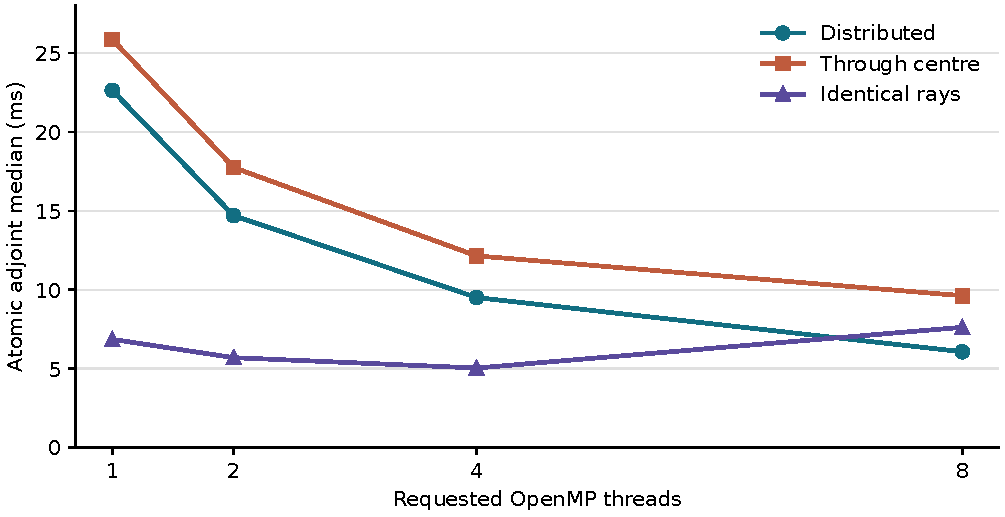
\includegraphics[width=.91\linewidth]{figures/atomic-adjoint.pdf}
\caption{Atomic-adjoint median time versus requested threads, from the
recorded experiment. Identical rays concentrate writes onto the same
voxels: eight threads were slower than four for this case. These curves
describe a single environment and benchmark, not confidence intervals.}
\end{figure}

The largest observed relative image difference from serial was
$7.1\times10^{-15}$ and the largest norm-scaled adjoint discrepancy
\eqref{eq:adjtest} was $1.1\times10^{-17}$. These are measured values,
not universal roundoff bounds. Geometry-dependent contention explains why
thread count should be measured rather than simply maximised.
The source experiment is \code{benchmarks/atomic_adjoint.py}; its recorded
JSON is \path{benchmarks/atomic_results_2026-10-27.json}. Both were added
in \atomiclink. Building the guide reads this JSON without rerunning the benchmark.

\subsection{Experimental oneMKL acceleration of cached operators on CSF3}
\label{sec:csf3-mkl}

An additional experiment on 27 October 2026 tested Intel oneMKL Sparse BLAS
on the University of Manchester CSF3 cluster. The benchmark-only adapter in
\path{benchmarks/mkl_probe.py} replaces products with a cached scalar CSR
matrix by oneMKL products, including products with six tensor components.
The LRT and TRT timings include the surrounding component packing,
contractions and transverse projections. These measurements concern cached
operators; they do not measure the matrix-free atomic backprojector or a
complete iterative reconstruction. The adapter remains experimental and
does not add a supported MKL backend to the package API.

Both repeated jobs requested 16 CPUs on one node and reported an AMD EPYC
9634 processor. They used Python 3.12.16, NumPy 2.3.5, SciPy 1.17.0 and
oneMKL 2026.2.0, with the GNU threading layer, LP64 indices and passive
OpenMP waiting. Each requested thread count ran in a fresh process;
dynamic OpenMP/MKL thread adjustment was disabled. The problem comprised
a $128^3$ grid and 100,000 random segments entering through one $x$-face
and leaving through the opposite face, with fixed random seed 20261027.
The scalar matrix had
21,200,180 nonzeros. This geometry is a performance test, not a claim of
adequate angular sampling for inversion.

Each product was evaluated before timing for a correctness check, followed
by nine timed repetitions with rotating and reversing backend order.
Table~\ref{tab:csf3-mkl} reports the sum of the separate forward and adjoint
median times. Geometry construction and backend preparation are excluded;
output allocation and the operator's per-call work are included. The
SciPy controls comprise the original CSR matrix, sorted CSR, and sorted
CSR with a separately cached CSR transpose. SciPy sparse products in these
controls are single-threaded.

\begin{table}[htbp]
\centering\small
\begin{tabular}{@{}r rrr rrr@{}}
\toprule
& \multicolumn{3}{c}{Run A} & \multicolumn{3}{c}{Run B} \\
\cmidrule(lr){2-4}\cmidrule(l){5-7}
MKL threads & Scalar & LRT & TRT & Scalar & LRT & TRT \\
\midrule
1  & 100.47 & 370.40 & 418.15 & 64.37 & 358.20 & 391.21 \\
2  &  32.64 & 224.82 & 244.77 & 39.81 & 206.22 & 261.47 \\
4  &  25.14 & 156.87 & 158.88 & 19.48 & 115.26 & 161.24 \\
8  &  20.01 &  97.06 & 134.44 & 12.39 &  77.22 & 117.38 \\
16 &  11.87 &  91.12 & 121.14 & 15.37 &  81.96 & 117.79 \\
\bottomrule
\end{tabular}
\caption{Cached-operator forward-plus-adjoint costs in milliseconds on
CSF3. Runs A and B are separate submissions of the same job script,
recorded in \texttt{mkl-23867575.json} and \texttt{mkl-23867786.json}.
Each entry sums two separate medians; it is not a measured solver iteration.
The two jobs had different permitted CPU sets. The raw files are archived
in \texttt{benchmarks/csf3/}.}
\label{tab:csf3-mkl}
\end{table}

For the eight-thread comparisons, the SciPy cached-transpose pair costs
were respectively $(106.26,588.70,625.17)$ ms in run A and
$(78.62,579.04,616.35)$ ms in run B, in scalar/LRT/TRT order. For the scalar
case this combines the sorted-CSR forward time with the cached-transpose
adjoint time. The corresponding gains from eight-thread MKL were
$5.31$ and $6.34$ for scalar products, $6.07$ and $7.50$ for LRT, and
$4.65$ and $5.25$ for TRT. These are within-run comparisons with that
specific single-threaded baseline.

The results support eight threads as a practical choice for this problem
size. Moving from eight to sixteen reduced LRT and TRT times by about
6\% and 10\% in run A, but increased them by about 6\% and 0.3\% in run B.
Thus sixteen threads showed no consistent tensor advantage. Variation
between jobs and the changed CPU affinity prevent a precise claim about
parallel efficiency or its hardware cause; these two runs do not establish
a universal optimum or a statistical confidence interval.

At eight threads, geometry construction took 0.50--0.58 s and additional
MKL preparation took 0.64--0.69 s. The process resident-memory increase
across MKL preparation was about 1.05 GiB, while the complete comparison
benchmark peaked at about 2.85 GiB. These measurements include allocations
beyond the original CSR matrix and should not be interpreted as the memory
required by a minimal MKL-only implementation. Charging the full MKL
preparation cost against the measured savings over the cached-transpose
baseline gives a break-even of approximately two LRT or TRT
forward/adjoint pairs; this excludes common geometry construction and
process/library startup.

Across both jobs the largest relative product discrepancy from SciPy was
$5.6\times10^{-16}$ or less, and the largest norm-scaled tensor adjoint
discrepancy was $4.2\times10^{-18}$ or less. This is evidence of agreement
for these discrete test problems, not of continuum reconstruction accuracy.
The measured speedups justify further evaluation of an optional cached
MKL backend, with complete reconstruction time and memory as the next
validation targets.

\section{Reproduction and scope for further work}
The guide's \code{README.md} gives a LaTeX build command and a script for
regenerating the figures. The following commands run the existing examples
and checks from the repository root in a suitable Python environment:
\par\noindent\begin{minipage}{\linewidth}
\begin{lstlisting}[language=bash]
python -m unittest discover -s tests -v
cmake -S . -B build/cpp
cmake --build build/cpp
ctest --test-dir build/cpp --output-on-failure
python examples/trt_slices.py --json
python benchmarks/benchmark.py
# With an OpenMP build:
python benchmarks/atomic_adjoint.py --threads 1 2 4 8
\end{lstlisting}
\end{minipage}\par
Optional dependency tests may skip if their software is missing; a passing
minimal installation is not evidence that CIL or ASTRA integration ran.
The CI configuration provisions these integrations separately and builds
the MATLAB MEX tests. Benchmarks report observations; they are not timing
gates on shared CI machines.

Useful next steps include a documented acquisition-geometry converter for
CIL, a separately tested TTRT adapter, additional external 3D comparisons,
and memory-controlled tensor operators for problems too large to cache.
Non-Abelian reconstruction needs physical measurement models and tested
Jacobian/adjoint pairs. More advanced tensor inversions require their own
specified data measure and sampling. ORT should receive a public definition
before an implementation is advertised. These are extensions of a common
geometric foundation, rather than capabilities implied by the present
examples.

\clearpage
\appendix
% SPDX-License-Identifier: Apache-2.0
\section{Exact-arithmetic specification and correctness}
\label{app:exact}

This is a first step towards formal verification: a precise specification
and a written mathematical proof of an exact-arithmetic model of
\code{walk()}. It is \textbf{not yet a machine-checked proof}, a proof about
the actual C++ floating-point execution, or a verification of the wrappers.
The correspondence below was checked against
\href{https://github.com/billlion/jacobsrays/blob/e1c4313550f86fd49547e7a9cb85f353d04f8a1d/include/jacobsrays/traverse.hpp}{\code{traverse.hpp} at revision \code{e1c4313}}.

A \emph{specification} states what a function must deliver, independently
of its implementation. A \emph{precondition} is an assumption on its inputs;
a \emph{postcondition} is a promised property of its output. A \emph{loop
invariant} is a statement that holds whenever execution reaches the top of
the loop. Proving an invariant requires establishing it initially and showing
that every iteration preserves it. Termination needs a separate argument.

\subsection{Inputs and the meaning of an output record}
\label{app:exact-contract}
Let $D\in\{2,3\}$. The preconditions are positive integers $n_a$, positive
real spacings $h_a$, and real origins $o_a$ and endpoints $p,e\in\mathbb R^D$,
where $0\leq a<D$. Define
\[
 r(t)=p+t(e-p),\qquad L=\|e-p\|_2,\qquad
 q_a=\frac{p_a-o_a}{h_a},\qquad v_a=\frac{e_a-p_a}{h_a}.
\]
The C++ core uses three coordinates; the 2D case embeds in it by adding a
stationary coordinate inside a single-cell slab.
Thus $q_a+t v_a$ is the ray coordinate in voxel units; $L$ is still a
physical length. The grid and its voxels are
\[
 \Omega=\prod_{a=0}^{D-1}[o_a,o_a+n_a h_a),\qquad
 V_c=\prod_{a=0}^{D-1}[o_a+c_a h_a,o_a+(c_a+1)h_a),
 \quad 0\leq c_a<n_a.
\]
These half-open boxes partition $\Omega$. In particular, a ray lying along
an internal face belongs to the higher-index cell in that coordinate.
The lower outer face is included and the upper outer face is excluded.

An output record $(c,a,b,\ell)$ denotes the portion with $a<t<b$ in voxel
$V_c$, with physical length $\ell=(b-a)L$. The implementation emits the
linear index $c_0+n_0(c_1+n_1c_2)$ in 3D, or $c_0+n_0c_1$ in 2D.
\textbf{The record need not own either endpoint as a point of its half-open
voxel.} For example, at $x=k$ a ray travelling towards decreasing $x$
enters cell $k-1$ immediately afterwards, although the point $x=k$ belongs
to cell $k$. Isolated endpoints have zero length.

The required postconditions are:
\begin{enumerate}
 \item If $L=0$, the output is empty. Otherwise, emit exactly one record for
 each voxel whose ray intersection has positive length, and no others.
 \item Each record has $0\leq a<b\leq1$, a valid cell index, and
 $r(t)\in V_c$ for every $a<t<b$. Its interval is the full positive-length
 intersection with that voxel, up to endpoints.
 \item Records occur in increasing parameter order. Consecutive intervals
 meet at an endpoint; their interiors are disjoint. Together they cover
 the part of the ray in $\Omega$, apart from finitely many endpoints.
 \item Each length is exact. In particular, writing $|S|$ for the
 one-dimensional measure of a parameter set,
 \[
   \ell_c=L\,|\{t\in[0,1]:r(t)\in V_c\}|,\qquad
   \sum_c\ell_c=L\,|\{t\in[0,1]:r(t)\in\Omega\}|.
 \]
 \item The algorithm terminates, with at most
 $1+\sum_a(n_a-1)$ emitted records when the output is nonempty.
\end{enumerate}
\subsection{The exact algorithm corresponding to the header}
\label{app:exact-algorithm}
Replace floating-point arithmetic by exact real arithmetic and fixed-width
indices by mathematical integers. Interpret \code{fma(first,v,q)} as
$q+\mathrm{first}\,v$, and the nested \code{hypot} calls as $L$.
The inactive-axis infinity is an ordered sentinel, used only in comparisons.
These replacements define the model; their correctness for machine
arithmetic is \emph{not} assumed to have been proved.
The callback is modelled as appending a record to a list. Any later proof
using an actual callback must specify its termination and effects on inputs.

Return immediately if $L=0$. For an axis with $v_a=0$, return empty if
$q_a\notin[0,n_a)$; otherwise it imposes no parameter restriction. For each
moving axis, form the closed slab interval with endpoints
$-q_a/v_a$ and $(n_a-q_a)/v_a$. Intersect these intervals with $[0,1]$,
calling the resulting lower and upper bounds $\alpha$ and $\beta$.
Return empty if $\alpha\geq\beta$.

Set $t=\alpha$, $x_a=q_a+\alpha v_a$, and initialise
\[
 c_a=\begin{cases}
       \lfloor x_a\rfloor,&v_a\geq0,\\
       \lceil x_a\rceil-1,&v_a<0,
     \end{cases}
 \qquad \sigma_a=\operatorname{sgn}(v_a).
\]
The next crossing parameter is
\[
 \tau_a=\begin{cases}
       (c_a+1-q_a)/v_a,&v_a>0,\\
       (c_a-q_a)/v_a,&v_a<0,\\
       +\infty,&v_a=0.
     \end{cases}
\]
While $t<\beta$, set $s=\min(\beta,\tau_0,\ldots,\tau_{D-1})$,
emit $(c,t,s,(s-t)L)$, and set $t=s$. If $s=\beta$, finish.
Otherwise, for \emph{every} axis with $\tau_a=s$, replace $c_a$ by
$c_a+\sigma_a$ and recompute $\tau_a$ using the formula above.

In the exact model, the header's clamps do not change the initial cell,
\code{stop > t} always holds in an entered loop iteration, and its early
out-of-grid return cannot occur before the final endpoint. The proof below
establishes these facts; they are not extra preconditions.

\subsection{Correctness proof}
\label{app:exact-proof}
\textbf{Theorem.} Under the preconditions above, the exact algorithm
satisfies all five postconditions.

\textbf{1. Clipping.}
If $v_a=0$, membership in that coordinate slab is constant and is exactly
the test $0\leq q_a<n_a$. If $v_a\ne0$, the inverse image of the closed
slab $[0,n_a]$ is the interval computed above. Replacing the actual half-open
slab by the closed slab changes membership only at its two endpoint
parameters. Hence, after the stationary-axis tests, the parameter set inside
the grid differs from the intersection of these closed intervals with
$[0,1]$ by at most finitely many points. It has positive length exactly when
$\alpha<\beta$. Every parameter strictly between these bounds lies in
$\Omega$. The empty returns, including point tangencies, are therefore
correct. The separately handled $L=0$ case has zero physical length.

\textbf{2. Initialisation.}
Assume now that $L>0$ and $\alpha<\beta$.
For $v_a>0$, clipping gives $0\leq x_a<n_a$: equality at the upper end
would leave no interior interval. Thus $\lfloor x_a\rfloor$ is a valid
cell, occupied immediately after $\alpha$. For $v_a<0$, similarly
$0<x_a\leq n_a$, and $\lceil x_a\rceil-1$ is the valid cell occupied
immediately after $\alpha$. For $v_a=0$, the stationary-axis test gives
$0\leq x_a<n_a$, and $\lfloor x_a\rfloor$ gives the prescribed ownership.
Both initial clamps in the header are consequently inactive.
For a moving axis, $\tau_a$ is strictly larger than $\alpha$ and is its
first cell-face crossing after $\alpha$.

\Needspace{12\baselineskip}
\textbf{3. Invariant.}
At the top of every entered iteration:
\begin{enumerate}[label=(\roman*)]
 \item $\alpha\leq t<\beta$, and the records already emitted correctly
 cover the parameter interval from $\alpha$ to $t$, up to endpoints.
 \item $c$ is a valid cell occupied immediately after $t$.
 \item Each moving axis has $\tau_a>t$, its first forward-in-parameter
 face crossing of this cell; stationary axes have $\tau_a=+\infty$.
\end{enumerate}
Here ``immediately after'' means that some $\varepsilon$ with
$0<\varepsilon\leq\beta-t$ exists such that $r(u)\in V_c$ for every
$u\in(t,t+\varepsilon)$. Initialisation proves the invariant before
the first iteration, with an empty output list.

\textbf{4. Preservation and the emitted interval.}
By (iii), $s>t$. No coordinate crosses a cell face for $t<u<s$, so the
entire open interval lies in $V_c$. Its physical length is exactly
$(s-t)L$. Appending it preserves ordered coverage and creates no overlap
of interiors. This is the maximal remaining interval in that cell:
at $s$ either the clipped ray ends or at least one coordinate leaves the cell.

If $s<\beta$, at least one moving axis has $\tau_a=s$.
Each such crossing is of an \emph{internal} plane: an outward crossing of
the outer box would end the clipped interval at or before $s$, contradicting
$s<\beta$. Updating every tied axis therefore gives valid indices and the
cell occupied immediately after $s$. A tied axis's next crossing increases
by $1/|v_a|>0$; untied axes already have $\tau_a>s$.
Thus (i)--(iii) hold for the next iteration. In particular, the header's
\code{next[a] <= stop} selects exactly the tied axes, and the early
out-of-grid return is unreachable here. Updating tied axes one at a time
within the update loop is harmless: no record is emitted between updates.

\textbf{5. Termination.}
The nonnegative integer
\[
 R(c)=\sum_{a:v_a>0}(n_a-1-c_a)+\sum_{a:v_a<0}c_a
\]
counts the internal planes still ahead, whether or not the finite ray will
reach them. Every nonfinal iteration decreases $R$ by the number of tied
axes, hence by at least one. This is a \emph{loop variant}: a quantity in
the nonnegative integers that strictly decreases on each continuation.
There cannot be infinitely many continuations. Since initially
$R\leq\sum_a(n_a-1)$, there are at most that many nonfinal iterations
and one final emission. The last emission ends at $\beta$.

\textbf{6. Completeness and uniqueness.}
The invariant and termination give contiguous coverage from $\alpha$ to
$\beta$, up to endpoints. Each moving cell coordinate only changes in its
fixed direction, and some coordinate changes between consecutive records;
therefore no cell can be visited twice. Every positive-length voxel
intersection contains an open parameter interval and so must be represented
in this coverage. Consequently the emitted records are exactly the required
intersections. Summing their lengths gives $L(\beta-\alpha)$, which equals
the length in the grid by the clipping argument. Valid cell coordinates
also imply a linear index between zero and $\prod_a n_a-1$ in mathematical
integer arithmetic. This proves all the postconditions.\hfill$\square$

\Needspace{18\baselineskip}
\subsection{A small example with a simultaneous crossing}
Take a $3\times2$ unit grid at the origin and
$p=(-1,-\tfrac12)$, $e=(4,2)$. Then
\[
 r(t)=(-1+5t,-\tfrac12+\tfrac52 t),\quad
 \alpha=\tfrac15,\quad\beta=\tfrac45,\quad L=\tfrac52\sqrt5.
\]
The exact output is
\begin{center}
\begin{tabular}{ccccc}
\toprule
Cell $c$ & Linear index & Entry $a$ & Exit $b$ & Length\\
\midrule
$(0,0)$ & $0$ & $1/5$ & $2/5$ & $\sqrt5/2$\\
$(1,0)$ & $1$ & $2/5$ & $3/5$ & $\sqrt5/2$\\
$(2,1)$ & $5$ & $3/5$ & $4/5$ & $\sqrt5/2$\\
\bottomrule
\end{tabular}
\end{center}
At $t=3/5$ the ray crosses $x=2$ and $y=1$ simultaneously, so both cell
coordinates advance. Cells $(2,0)$ and $(1,1)$ receive no positive-length
interval. The initial variant is $R=2+1=3$; the first crossing reduces it
to $2$ and the simultaneous crossing reduces it to $0$. The next record
ends at the grid boundary. Reversing the ray reverses the cell list and
maps every interval $(a,b)$ to $(1-b,1-a)$, preserving its length.

\subsection{What remains to be formalised}
The first Lean milestone would be the one-coordinate initialisation and
next-crossing lemmas, followed by the invariant and the decreasing integer
$R$. These statements involve exact arithmetic and order, not a numerical
error analysis. For rational input data, all clipping and crossing parameters
are rational; the generally irrational common factor $L$ can be handled
separately. A Lean model must still be linked to the stated algorithm, and
its proof must contain no unproved placeholders before being called checked.

The current proof does not cover rounding, near ties, overflow/underflow,
the C++ validators or casts, library-function accuracy, callback behaviour,
parallel accumulation, or Python/MATLAB memory handling. The output
cardinality bound and index bound above are over mathematical integers;
fixed-width implementations require further proofs. Comparing a reference
model with C++ would add useful tests, but would not establish their
equivalence for all inputs. That equivalence and a floating-point contract
are later milestones, separate from the exact theorem proved here.


\clearpage
\addcontentsline{toc}{section}{References}
\interlinepenalty=10000
\bibliographystyle{plainnat}
\bibliography{references}
\end{document}
